\noindent
Si fa ora un esempio su due campi vettoriali definiti su un domimio non semplicemente connesso, cioè dove tutti i percorsi chiusi sono riducibili a un punto. Entrambi hanno rotore nullo all'interno del dominio, ma solo uno dei due è conservativo.
\begin{exercise}
Dati i seguenti campi vettoriali
\begin{equation}
 \bm{F}_1 =   \frac{x}{x^2+y^2} \bm{\hat{x}} + \frac{y}{x^2+y^2} \bm{\hat{y}} \qquad , \qquad
 \bm{F}_2 = - \frac{y}{x^2+y^2} \bm{\hat{x}} + \frac{x}{x^2+y^2} \bm{\hat{y}}
\end{equation}
si chiede di
\begin{enumerate}

\item definire il dominio e 'disegnare' i campi vettoriali;

\item calcolare il rotore, la divergenza e (se esiste) la funzione $\phi$ t.c. $\bm{F} = \bm{\nabla}\phi$;

\item calcolare la circuitazione ($\Gamma = \oint_l \bm{F} \cdot \bm{\hat{t}}$)  sulle
 circonferenze di raggio unitario $C$ centrata in $(0,0)$ e $C'$ centrata in $(2,1)$;

\item calcolare il flusso ($\Phi = \oint_l \bm{F} \cdot \bm{\hat{n}}$) uscente dalle curve $C$ e $C'$;	

\item calcolare l'integrale $\int_\gamma \bm{F}_2 \cdot d\bm{r}$ su una curva $\gamma$ che 
 avvolge due volte l'origine in senso antiorario.

\end{enumerate}
\end{exercise}


\begin{enumerate}

\item Il dominio $\Omega$ dei due campi vettoriali è $\mathbb{R}^2\backslash\{ 0 \}$: non è semplicemente connesso.

  \textit{Osservazione}. A differenza di $\mathbb{R}^2\backslash\{ 0 \}$, $\mathbb{R}^3\backslash\{ 0 \}$ 
    è semplicemente connesso (perchè?).

  \textit{Grafici...}

\item 

\begin{itemize}

\item{Rotore}:
all'interno del dominio $\Omega$ il rotore dei due campi vettoriali è nullo. 
Infatti, la componente lungo $z$ è l'unica che può essere non nulla, poichè il campo è definito nel piano $xy$ e dipende solo da $x$ e $y$.
\begin{equation}
\begin{aligned}
  \frac{\partial F_{1y}}{\partial x} - \frac{\partial F_{1x}}{\partial y} = -\frac{2xy}{(x^2+y^2)^2} + \frac{2xy}{(x^2+y^2)^2} = 0 \\
  \frac{\partial F_{2y}}{\partial x} - \frac{\partial F_{2x}}{\partial y} =  \frac{y^2-x^2}{(x^2+y^2)^2} - \frac{y^2-x^2}{(x^2+y^2)^2} = 0 
\end{aligned}
\end{equation}

\item{Divergenza}:
all'interno del dominio $\Omega$ la divergenza dei due campi vettoriali è nullo. 

\textit{(...)}

\item{$\phi$}:
all'interno del dominio $\Omega$, le funzioni $\phi$, a meno 
di una costante (ininfluente) valgono
\begin{equation}
 \phi_1 = \frac{1}{2} \ln(x^2 + y^2) \qquad , \qquad \phi_2 = \text{atan} \displaystyle\left(\frac{y}{x}\right) \ .
\end{equation}

Ad esempio per il campo $\bm{F}_1$, si può scirvere la relazione $\bm{F} = \bm{\nabla}\phi$ in coordinate cartesiane
\begin{equation}
  \frac{\partial \phi}{\partial x} = \frac{x}{x^2+y^2} \quad , \quad
  \frac{\partial \phi}{\partial y} = \frac{y}{x^2+y^2} \ . 
\end{equation}
Integrando la prima in x e la seconda in y:
\begin{equation}
\begin{aligned}
  \phi(x,y) = \int \frac{x}{x^2+y^2} dx = \int \frac{1}{x^2+y^2}d(x^2+y^2) = \frac{1}{2} \ln (x^2+y^2) + f(y) \\
  \phi(x,y) = \int \frac{x}{x^2+y^2} dy = \int \frac{1}{x^2+y^2}d(x^2+y^2) = \frac{1}{2} \ln (x^2+y^2) + g(x) \\ 
\end{aligned}
\end{equation}

dove compaiono le funzioni $f(y)$ e $g(x)$, che tengono conto dell'arbitrarietà dell'integrale di una derivata parziale: si pensi di fare
la derivata parziale delle relazioni appena trovate. Derivando la prima rispetto a $x$ si ha:
\begin{equation}
  \frac{\partial \phi}{\partial x} = \frac{\partial}{\partial x} \displaystyle\left(\frac{1}{2} \ln (x^2+y^2)\right) + 
               \frac{\partial f(y)}{\partial x} = \frac{x}{x^2+y^2} + 0
\end{equation}
La derivata $\frac{\partial f(y)}{\partial x}$ è identicamente nulla, poichè la funzione $f(y)$ non dipende da $x$.
Da un confronto tra le due forme di $\phi$, segue che $f(y)$ e $g(x)$ devono essere uguali e costanti: il valore di questa costante
additiva è comunque ininfluente ai termini della definizione di un potenziale.

\end{itemize}

\item 
\begin{itemize}

\item{Circuitazione su $C'$}:
entrambi gli integrali calcolati su $C'$ sono nulli, poichè il percorso di integrazione è una linea 
 chiusa che non circonda l'origine ma una regione semplicemente connessa nella quale il campo ammette
 potenziale. In altre parole, $C'$ circonda una regione del dominio che è semplicemente connessa ed è
 possibile applicare direttamente il teorema del rotore, avendo definito $R'$ come la parte del dominio interna a $C'$,
\begin{equation}
  \Phi = \oint_{C'} \bm{F} \cdot \bm{\hat{t}} = \int_{R'} [\bm{\nabla} \times \bm{F}] \cdot \bm{\hat{n}} = 0 \ ,
\end{equation}
poichè il rotore è nullo in tutto $\Omega$ e quindi anche in $R' \subset \Omega$.

\item{Circuitazione su $C'$}: $C$ invece circonda l'origine, causa della non semplice connessione
 del dominio; una diretta applicazione del teorema del rotore non è quindi possibile;
 gli integrali su $C$ devono essere calcolati e valgono
\begin{equation}
I_1 = \oint_C \bm{F}_1 \cdot d\bm{r} = 0 \qquad , \qquad
I_2 = \oint_C \bm{F}_2 \cdot d\bm{r} = 2 \pi
\end{equation}

I due integrali possono essere calcolati facilmente in coordinate polari. L'elemento $d\bm{r}$ sulla circonferenza di raggio $r$ è $d\bm{r} = r d\theta \bm{\hat{\theta}}$.
I due campi possono essere scritti in coordinate polari come:
\begin{equation}
  \bm{F}_1 = \frac{1}{r} \bm{\hat{r}} \qquad , \qquad   \bm{F}_2 = \frac{1}{r} \bm{\hat{\theta}} 
\end{equation}

Si può notare che il campo $\bm{F}_1$, calcolato sul contorno, è sempre perpendicolare ad esso. Il primo integrale è quindi nullo.
\begin{equation}
\begin{aligned}
  I_{1C} = \int_C \bm{F}_1 \cdot d\bm{r} = \int_{\theta=0}^{2\pi} \bm{\hat{r}} \cdot \bm{\hat{\theta}} d\theta = 
           \int_{\theta=0}^{2\pi} 0 d\theta = 0 \\
  I_{2C} = \int_C \bm{F}_2 \cdot d\bm{r} = \int_{\theta=0}^{2\pi} \bm{\hat{\theta}} \cdot \bm{\hat{\theta}} d\theta = 
           \int_{\theta=0}^{2\pi} d\theta = 2\pi \\
\end{aligned}
\end{equation}	

\end{itemize}

\item
\begin{itemize}
\item{Flussi su $C'$}: Poichè $R'$ (vedi sopra) è semplicmente connesso, si può applicare il teorema
 della divergenza. I flussi di entrambi i campi su $C'$ sono nulli, poichè la divergenza dei due campi
 è nulla in tutto il dominio $\Omega$.

\item{Flussi su $C$}:  $C$ invece circonda l'origine, causa della non semplice connessione
 del dominio; una diretta applicazione del teorema della divergenza non è quindi possibile;
 gli integrali su $C$ devono essere calcolati e valgono
\begin{equation}
 \Phi_{C1} = \oint_C \bm{F}_1 \cdot d\bm{n} = 2 \pi \qquad , \qquad
 \Phi_{C2} = \oint_C \bm{F}_2 \cdot d\bm{n} = 0  \ .
\end{equation}

\end{itemize}

\item L'integrale di $\int_\gamma \bm{F}_2 \cdot d\bm{r}$ vale $4\pi$.

\begin{itemize}

\item
 Se la circuitazione calcolata sul contorno $C$ vale $\Gamma$ ($2\pi$ nel caso dell'esercizio), la
 circuitazione calcolata su qualsiasi altra curva $l$ che avvolge l'origine una sola volta avrà lo stesso valore.
 Infatti, se viene introdotto il 'taglio' $\gamma_c$ (invalicabile), si ottiene che il dominio 'tagliato' è
 semplicemente connesso e la circuitazione sul suo contorno ($\l \cup \gamma_c \cup C^- \cup \gamma_c^- $) è
 nulla, dove con $C^-$ si è indicata la circonferenza percorsa in senso orario. Ricordando che i contributi su $
 \gamma_c$ si annullano a
 vicenda e che se si inverte il verso di percorrenza di una curva la circuitazione cambia segno
\begin{equation}
 0 = \int_{l \cup \gamma_c \cup C^- \cup \gamma_c^- } \bm{F} \cdot d\bm{r} = 
 \int_{l} \bm{F} \cdot d\bm{r} + \int_{\gamma_c} \bm{F} \cdot d\bm{r} +
 \int_{C^-} \bm{F} \cdot d\bm{r} + \int_{\gamma_c-} \bm{F} \cdot d\bm{r} = 
 \int_{l} \bm{F} \cdot d\bm{r} - \int_{C} \bm{F} \cdot d\bm{r} \ ,
\end{equation}
%
e quindi $ \int_{l} \bm{F} \cdot d\bm{r} = \int_{C} \bm{F} \cdot d\bm{r} = \Gamma $.
%
\vspace{-0.5cm}
\begin{figure}[h!]
\centering
%\captionsetup[subfigure]{labelformat=empty}
\subfloat[][\emph ]
   {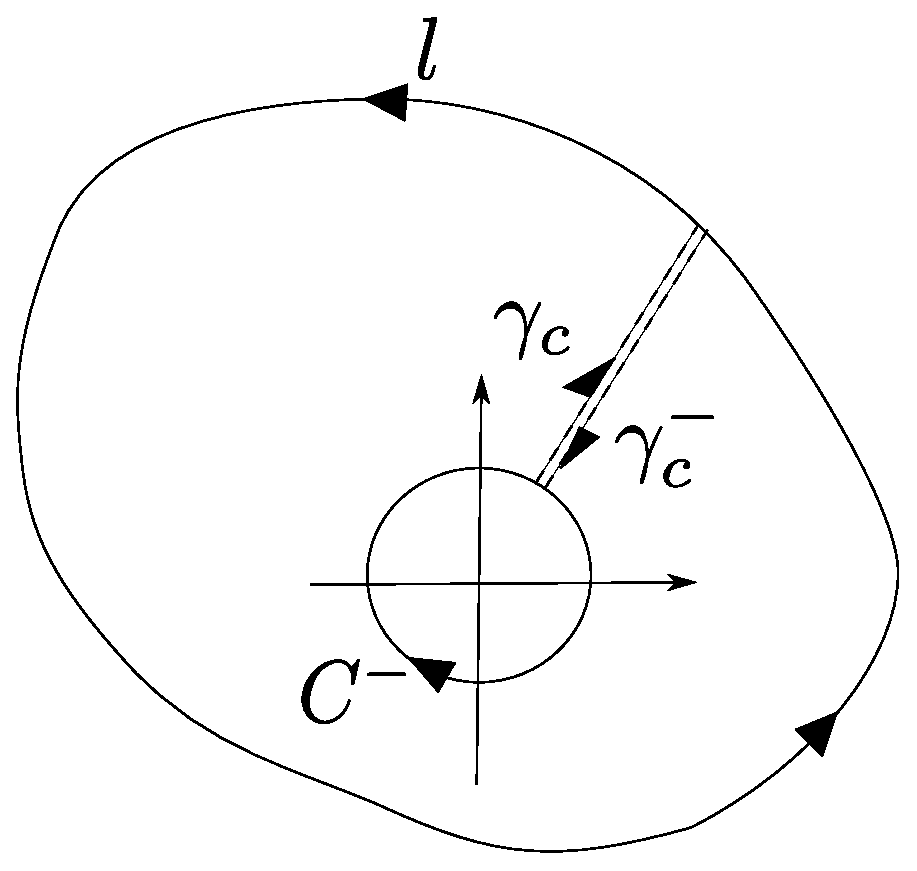
\includegraphics[width=0.26\textwidth]{./fig/Generale.eps}} \qquad
\subfloat[][\emph ]
   {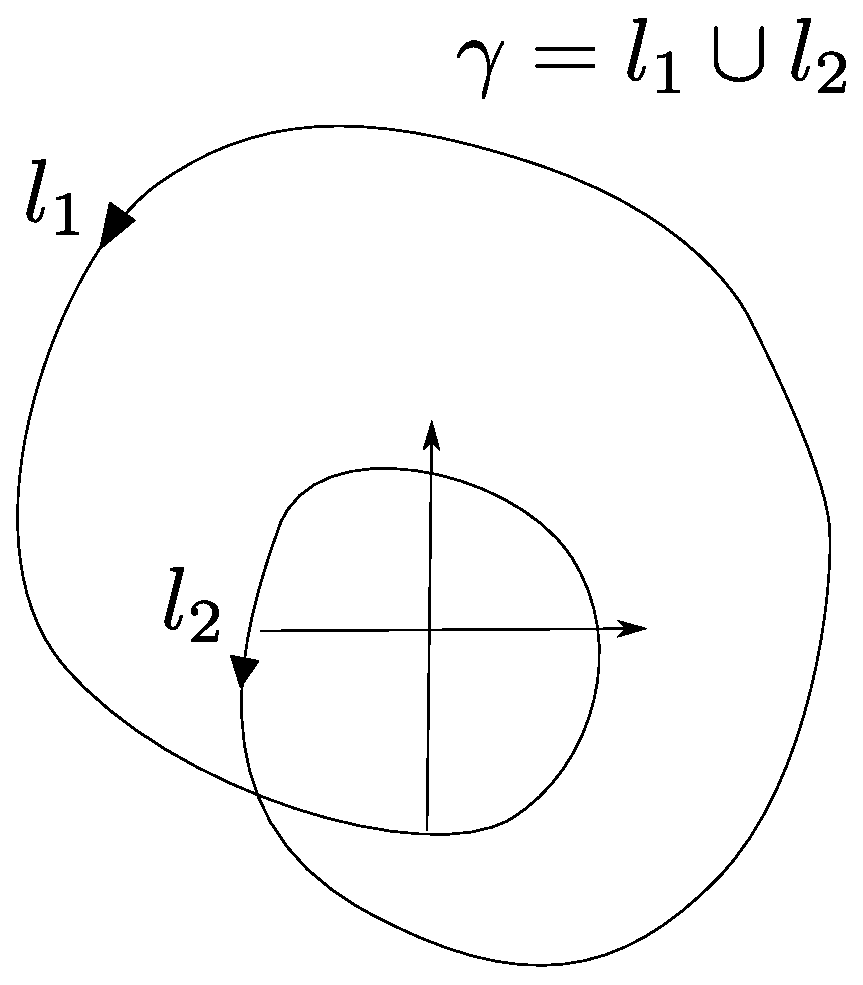
\includegraphics[width=0.26\textwidth]{./fig/AvvDue.eps}} \qquad
\subfloat[][\emph  ]
   {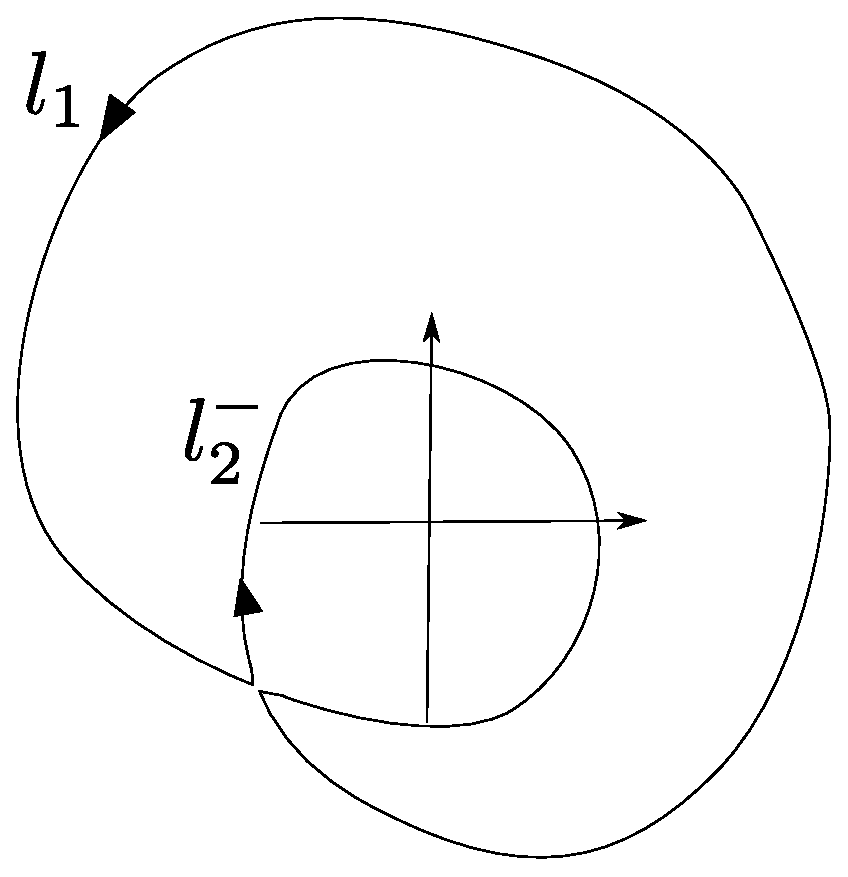
\includegraphics[width=0.26\textwidth]{./fig/AvvDue2.eps}}
\end{figure}

\item
 Ora il percorso $\gamma$ può essere 'suddiviso' nelle curve $l_1$, $l_2$. Si può definire ora la curva 
 composta da $l_1$ e $l_2^-$ (il verso è importante!!).
 Con ragionamenti analoghi a quelli fatti in precedenza:
\begin{equation}
 0 = \int_{l_1 \cup l_2^-} \bm{F} \cdot d\bm{r} = 
 \int_{l_1} \bm{F} \cdot d\bm{r} - \int_{l_2} \bm{F} \cdot d\bm{r}
\end{equation}

Da questo si ricava che $\int_{l_1} \bm{F} \cdot d\bm{r} = \int_{l_2} \bm{F} \cdot d\bm{r} = \Gamma$. Poichè
l'integrale su $\gamma$ è la somma dei due integrali, si ottiene:

\begin{equation}
 \int_{l} \bm{F} \cdot d\bm{r} = \int_{l_1 \cup \l_2} \bm{F} \cdot d\bm{r} = 
  \int_{l_1} \bm{F} \cdot d\bm{r} +  \int_{l_2} \bm{F} \cdot d\bm{r} = 2 \Gamma = 4 \pi
\end{equation}

\end{itemize}

\end{enumerate}


\begin{figure}[h]
\centering
%\captionsetup[subfigure]{labelformat=empty}
\subfloat[][\emph Percorsi di integrazione dell'esercizio. $C$ avvolge una volta sola in 'buco' nel dominio, $C'$ mai, $\gamma$ due volte.]
   {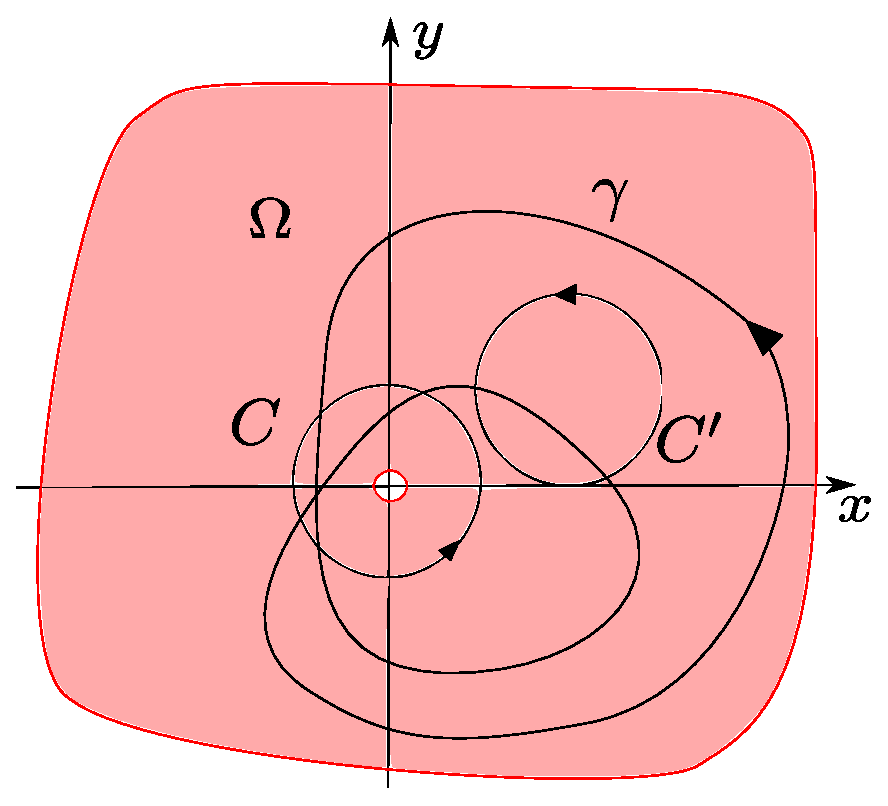
\includegraphics[width=0.40\textwidth]{./fig/IntPath.eps}} \qquad
\subfloat[][\emph Integrale su un percorso non riducibile. Il dominio $R$ (in rosa) non è semplicemente connesso. Si può dimostrare che
  se l'integrale $I_1$ definito su un percorso 'che circonda' una sola volta 'il buco' all'interno del dominio $I_1 = \oint_{l_1} \bm{F} \cdot d \bm{r} = \Gamma$, allora l'integrale $I$ definito su $\gamma$ che circonda $N$ (indice di avvolgimento) volte 'il buco' nello stesso verso di $l_1$, vale
$I_1 = \oint_{l_1} \bm{F} \cdot d \bm{r} = N \Gamma$. ]
   {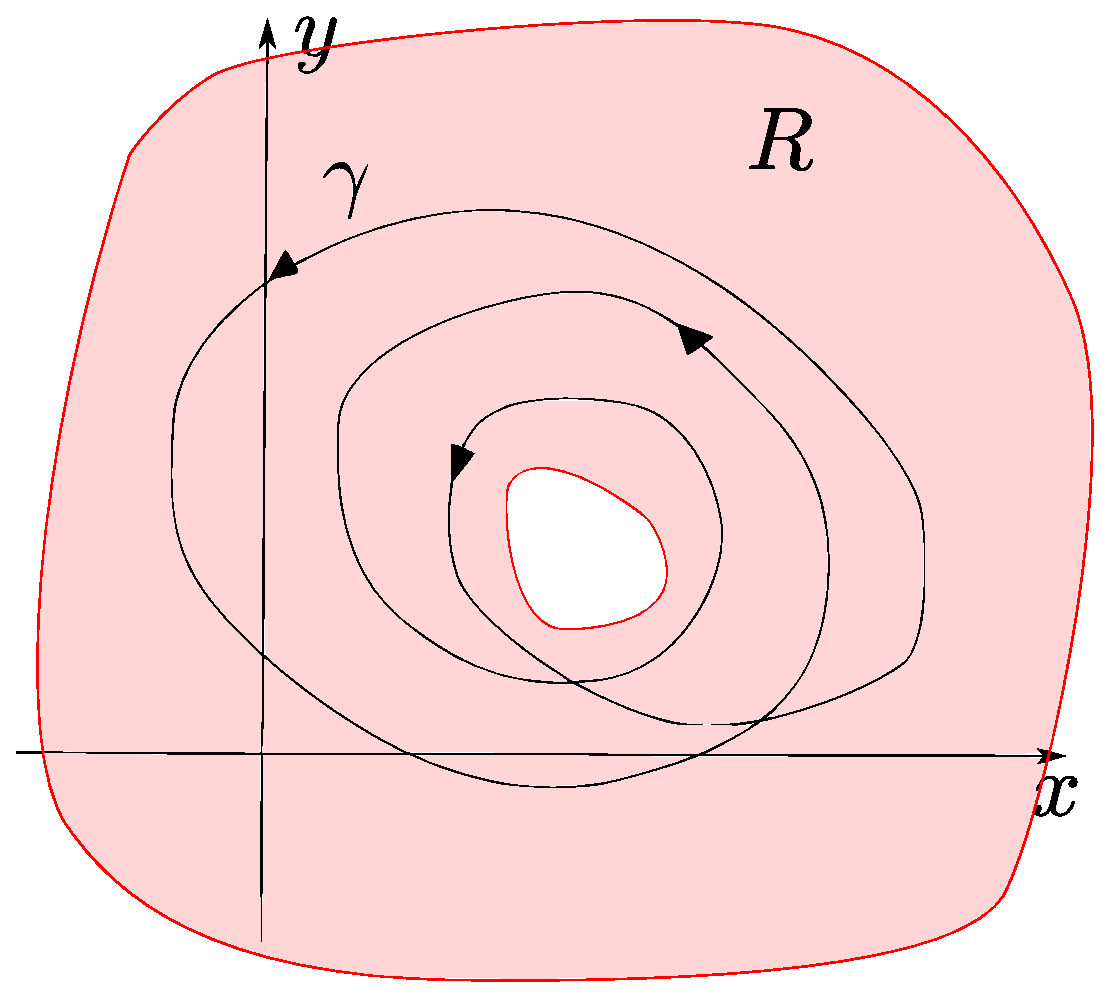
\includegraphics[width=0.40\textwidth]{./fig/IndiceAvvolgimento.eps}}
\end{figure}

